\documentclass{article}

    % the title part of the article.
    % use \maketitle after \begin{document} to make the title.
    \title{test}
    \author{charliezhao}
    \date{June 2018}

    % import packages listed in package.sty.
    \usepackage{package}

    \begin{document}

        % make the title with the details above.
        \maketitle

        % start a new page.
        \newpage

        % create contents for the article.
        \tableofcontents

        \newpage

        % split the whole article into small parts
        % which are stored separately in different tex files.
        % use \input to import the tex file into the article.
        \begin{abstract}
    There is a theory which states that if ever anyone discovers 
    exactly what the Universe is for and why it is here, 
    it will instantly disappear and be replaced by something even more bizarre and inexplicable.
    There is another theory which states that this has already happened.
\end{abstract}
        \section{Introduction}
    There is a theory which states that if ever anyone discovers 
    exactly what the Universe is for and why it is here, 
    it will instantly disappear and be replaced by something even more bizarre and inexplicable.
    There is another theory which states that this has already happened.
    % use citep to cite the reference in the bib file.
    % the index is shown at the first place in its reference
    % and should be in the {}.
    \citep{adams1995hitchhiker}
    There is a theory which states that if ever anyone discovers 
    exactly what the Universe is for and why it is here, 
    it will instantly disappear and be replaced by something even more bizarre and inexplicable.
    There is another theory which states that this has already happened.
    There is a theory which states that if ever anyone discovers 
    exactly what the Universe is for and why it is here, 
    it will instantly disappear and be replaced by something even more bizarre and inexplicable.
    There is another theory which states that this has already happened.
    \citep{adams1995hitchhiker2}
        \begin{multicols}{2}
    There is a theory which states that if ever anyone discovers 
    exactly what the Universe is for and why it is here, 
    it will instantly disappear and be replaced by something even more bizarre and inexplicable.
    There is another theory which states that this has already happened.
    There is a theory which states that if ever anyone discovers 
    exactly what the Universe is for and why it is here, 
    it will instantly disappear and be replaced by something even more bizarre and inexplicable.
    There is another theory which states that this has already happened.
\end{multicols}

\begin{multicols}{3}
    There is a theory which states that if ever anyone discovers 
    exactly what the Universe is for and why it is here, 
    it will instantly disappear and be replaced by something even more bizarre and inexplicable.
    There is another theory which states that this has already happened.
    There is a theory which states that if ever anyone discovers 
    exactly what the Universe is for and why it is here, 
    it will instantly disappear and be replaced by something even more bizarre and inexplicable.
    There is another theory which states that this has already happened.
\end{multicols}
        % insert figures into the article.
% 'h' to put the figure at the right place.
% 't' to put the figure at the top of the page.
% 'b' to put the figure at the bottom of the page.
% 'p' to create a blank page for the figure.
\begin{figure}[h!]
    \centering
    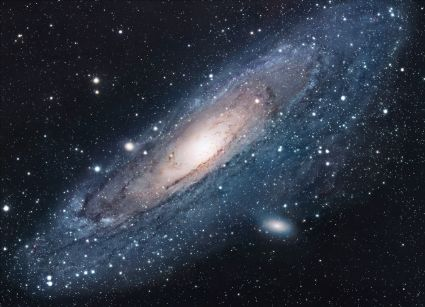
\includegraphics[height=5cm ,width=8cm,angle=0]{universe.jpg}
    \caption{The Universe}
    \label{fig:universe}
\end{figure}

% insert multiple figures in a group into the article.
\begin{figure}[t!]
    \centering
    \subfigure[1st] {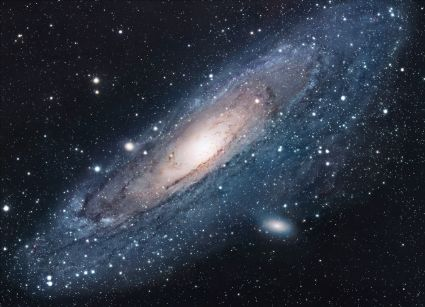
\includegraphics[height=2in,width=2in,angle=-90]{universe.jpg}}
    \subfigure[2nd] {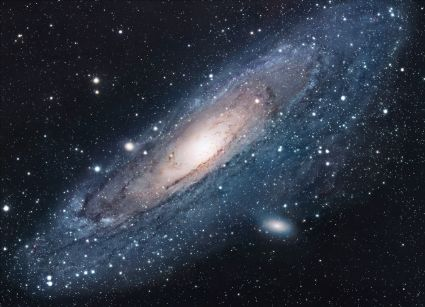
\includegraphics[height=2in,width=2in,angle=-90]{universe.jpg}}
    \subfigure[3rd] {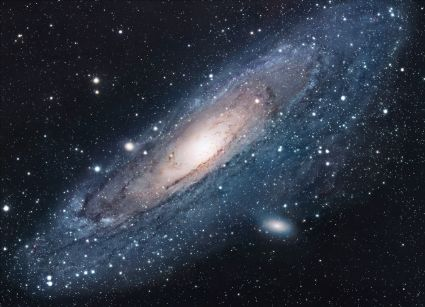
\includegraphics[height=2in,width=2in,angle=-90]{universe.jpg}}
    \caption{The Universe}
    \label{fig:universe2}
\end{figure}
        \section{Conclusion}
    There is a theory which states that if ever anyone discovers 
    exactly what the Universe is for and why it is here, 
    it will instantly disappear and be replaced by something even more bizarre and inexplicable.
    There is another theory which states that this has already happened.
    \citep{adams1995hitchhiker}
    There is a theory which states that if ever anyone discovers 
    exactly what the Universe is for and why it is here, 
    it will instantly disappear and be replaced by something even more bizarre and inexplicable.
    There is another theory which states that this has already happened.
    There is a theory which states that if ever anyone discovers 
    exactly what the Universe is for and why it is here, 
    it will instantly disappear and be replaced by something even more bizarre and inexplicable.
    There is another theory which states that this has already happened.
    \citep{adams1995hitchhiker2}

        % set style for the references.
        % plain style prints the names without abbreviations.
        % abbrv style prints the opposite.
        % the list is stored in reference.bib.
        \bibliographystyle{plain}
        \bibliography{reference}

    \end{document}
